A method to provide an estimate of the contribution of \ttbar with
fake \tauhad is provided by the so called scale factor (SF) method. Another method
explored by the analysis, the fake-rate method, is described in Appendix~\ref{subsec:ttbarfake}.
The general idea of the fake rate method and the scale factor method is similar. The main
difference is that the scale factor method aims to measure data-driven
corrections (i.e.\ the scale factor) for fake \tauhad passing identification in
\ttbar MC simulation, while the fake rate method aims to measure the efficiency
of tau identification directly. As a result, the scale factor method only
requires well-calibrated \tauhad candidates after passing loose identification,
wheras the fake rate method relies on \tauhad candidates without identification.
This allows to produce histograms for the SF measurement with full experimental
and modelling uncertainties\footnote{This is infeasible for the fake rate
  method, since the size of CxAODs becomes intractable when not requiring
  Tau-ID.} and therefore the SFs can be measured using a full profile likelihood
fit. Due to the additional degrees of freedom in the fit, including \ttbar
modelling uncertainties, the reweighting of the \ttbar MC is not applied for
this method.

The region used for the fake \tauhad scale factor measurement uses the
$\taulep\tauhad$-channel selection:
\begin{itemize}
\item \tauhad passing loose ID and 2 b-tags
\item Only events passing the single lepton triggers are considered
\item OS charge for $\ell$ \& \tauhad
\item $m_{bb} > \SI{150}{\GeV}$ ensuring orthogonality with the $\taulep\tauhad$
  signal region
\item $\tauhad \, \pT > \SI{25}{\GeV}$
\item \tauhad $\left|\eta\right| < 2.5$ instead of 2.3 to harmonize with the
  $\tauhad\tauhad$ selection
\end{itemize}

The scale factors need to be measured for multiple levels of \tauhad
identification due to different, trigger-dependent combinations of
offline and HLT \tauhad identification used in the
$\tauhad\tauhad$-channel. The following summarizes the four
combinations of offline and HLT \tauhad identification that are
considered and their relevance for the $\tauhad\tauhad$ event
selection:
\begin{itemize}
\item Loose offline \tauhad ID only:\\
  Subleading fake \tauhad in STT events
\item Loose offline \tauhad ID + \verb|HLT_tau25_medium1_tracktwo|:\\
  Fake \tauhad in DTT events (2015 - 2017)
\item Loose offline \tauhad ID + \verb|HLT_tau25_medium1_tracktwoEF|:\\
  Fake \tauhad in DTT events (2018 until period K)
\item Loose offline \tauhad ID + (\verb|HLT_tau25_medium1_tracktwoEF|
  \textbf{or} \verb|HLT_tau25_mediumRNN_tracktwoMVA|):\\
  Fake \tauhad in DTT events (2018 from period K)
\end{itemize}
These combinations resemble the triggers used in the
$\tauhad\tauhad$-channel which are described
in~\Cref{sec:hadhad_trigger_selection}. Scale factors for these
combinations are measured in fits of the SF-CR described above.

For the measurement of scale factors after HLT \tauhad-identification,
the loose \tauhad candidates entering the fit are also required to
match the corresponding single-\tauhad trigger leg. For data the
matching is performed to the corresponding resurrected trigger. Based
on the period-dependent availability of the triggers, different
datasets are used for fitting:
\begin{itemize}
\item \verb|HLT_tau25_medium1_tracktwo|: Available for the full Run 2
  dataset (ca.\ 139 fb$^{-1}$)
\item \verb|HLT_tau25_medium1_tracktwoEF|: Available only for 2018 data /
  MC16E (ca.\ 58 fb$^{-1}$)
\item \verb|HLT_tau25_mediumRNN_tracktwoMVA|: Available from 2018 period K (ca.\ 37 fb$^{-1}$)
\end{itemize}

In previous versions of this note, separate scale factors were
measured for single-\tauhad triggers with a HLT \tauhad \pT threshold
of \SI{35}{\GeV}, which corresponds to the trigger-leg for the leading
\tauhad in DTT events, in addition to the \SI{25}{\GeV} threshold
triggers. These triggers use the same \tauhad identification algorithm
and only differ in the \tauhad \pT threshold at the HLT.  Therefore,
after applying the offline threshold corresponding to the
\verb|HLT_tau35| triggers of \SI{40}{\GeV}, the events selected by
both triggers overlap significantly. The overlap is checked using
simulated \ttbar events with fake \tauhad in the scale factor
measurement region. After the offline threshold applied by the
analysis, about \SI{95}{\percent} (\SI{85}{\percent}) of 1-prong
(3-prong) fake \tauhad events in \ttbar are selected by both
triggers. The overlap further increases with increasing \tauhad
\pT. Moreover, comparing the measured scale factors for both HLT
thresholds shows no significant difference outside of the measurement
uncertainties. Therefore, the measurement is only performed for the
relevant \verb|HLT_tau25| triggers and the scale factors are also
applied to fake \tauhad matched to \verb|HLT_tau35| triggers. An
additional benefit of this approach is the proper treatment of the
large correlation originating from the overlap of both triggers.
Plots reinforcing this decision can be found
in~\Cref{subsec:appendix_bkg_ttbar_fake_sf} (i.e.\
\Cref{fig:ttbar_hadhad_sf_correlation_triggers,fig:ttbar_hadhad_sf_idfit_tau25_tau35}). An
uncertainty is assigned for \ttbar events where the leading \tauhad
candidate is faked by a jet to account for this approximation. This
uncertainty is applied for fake 1-prong \tauhad up to \SI{50}{\GeV}
and fake 3-prong \tauhad up to \SI{60}{\GeV}. Beyond these thresholds
the \tauhad candidates are sufficiently far away from the
trigger-thresholds such that the difference between the triggers is
negligible. The size of the uncertainty is derived by comparing the
nominal scale factor measurement with an alternative measurement where
events are required to match the equivalent HLT\_tau35
triggers. In~\Cref{tab:ttbarfake_hadhad_tau25tau35_uncertainty} the
approximate size of these uncertainties are summarized. The shape
impact of these uncertainties are propagated to the fit. The overall
normalization impact of these uncertainties on the estimate of \ttbar
with a leading fake \tauhad is small (less than 0.5 \%) after
integrating over the \tauhad \pT spectrum of the leading fake \tauhad
candidate in \ttbar.

\begin{table}[htb]
  \centering
  \begin{tabular}{lrr}
    \toprule
    & 1-prong \tauhad & 3-prong \tauhad \\
    & (40 - 50 GeV) & (40 - 60 GeV) \\
    \midrule
    HLT\_tauXX\_medium1\_tracktwo (ttbarFT) & $\pm 5.8 \%$ & $\pm 5.5 \%$ \\
    HLT\_tauXX\_medium1\_tracktwo (ttbarFF) & $\pm 5.9 \%$ & $\pm 5.2 \%$ \\[0.5em]

    HLT\_tauXX\_medium1\_tracktwoMVA (ttbarFT) & $\pm 6.4 \%$ & $\pm 8.1 \%$ \\
    HLT\_tauXX\_medium1\_tracktwoMVA (ttbarFF) & $\pm 6.4 \%$ & $\pm 8.0 \%$ \\[0.5em]

    HLT\_tauXX\_mediumRNN\_tracktwoMVA (ttbarFT) & $\pm 3.8 \%$ & $\pm 2.7 \%$ \\
    HLT\_tauXX\_mediumRNN\_tracktwoMVA (ttbarFF)& $\pm 4.0 \%$ & $\pm 2.6 \%$ \\
    \bottomrule
  \end{tabular}

  \caption{Uncertainty on \ttbar events with a leading fake \tauhad
    derived from comparing measured HLT\_tau25 and HLT\_tau35 scale
    factors close to the trigger threshold. The uncertainty is given
    relative to the leading \tauhad \pT bin where it is applied. The
    total uncertainty on the fake \ttbar estimate is small (less than
    0.5 \%) after integrating over the leading \tauhad \pT spectrum in
    \ttbar.}
  \label{tab:ttbarfake_hadhad_tau25tau35_uncertainty}
\end{table}

The scale factors are measured in regions described by the prongness and \pT of
the \tauhad candidate:
\begin{itemize}
\item 1-prong \tauhad \pT (GeV): $(25, 30)$, $(30, 35)$, $(35, 40)$, $(40, 45)$, $(45, 55)$, $(55,
    70)$, $(70, \infty)$
\item 3-prong \tauhad \pT (GeV): $(25, 30)$, $(30, 40)$, $(40, 50)$, $(50, 70)$,
  $(70, \infty)$
\end{itemize}
these regions are primarly determined by the available statistics and
the \tauhad \pT thresholds applied due to the \tauhad triggers. The
fit uses a dedicated floating parameter (the fake scale factor) in
every region scaling the yield of \ttbar with a fake \tauhad from MC
in that particular region. At the same time the inclusive \ttbar
normalisation is varied using another floating parameter (i.e.\ a
single free parameter for a given fit). To disentangle the effect of
the fake \tauhad SF and the \ttbar normalisation \mtw is used as a
discriminant between \ttbar with true and fake \tauhad\footnote{In a
  previous version of the note a pseudo-continuous binning in
  \tauhad-ID was used but this is not officially supported by the
  Tau-WG and therefore replace by the \mtw approach.}. Events with a
true \tauhad and a lepton originate from dileptonic \ttbar which
features a long tail towards high \mtw. In contrast, events containing
a fake \tauhad and a lepton show soft bound on \mtw at the W-mass
since fake \tauhad in \ttbar primarily originate from quarks of the
W-decay in semileptonic decays of the \ttbar system.

Exemplary pre-fit distributions illustrating the discriminant and two
\tauhad \pT / prong regions are shown
in~\Cref{fig:ttbarfake_hadhad_prefit}. A pre-fit summary of regions
entering the fit is shown in~\Cref{fig:ttbarfake_hadhad_prefit_summary}.

\begin{figure}[htb]
  \centering
  \subfloat[]{\includegraphics[width=0.42\textwidth]{figures/bkg/hadhad_ttbar_fakes/scale_factor_method/TauPt4045_1P}}
  \subfloat[]{\includegraphics[width=0.42\textwidth]{figures/bkg/hadhad_ttbar_fakes/scale_factor_method/TauPt4050_3P}}
  \caption{Pre-fit distribution in the 1-prong $\SI{40}{\GeV} \leq \tauhad \,
    \pT < \SI{45}{\GeV}$ region (a) and the 3-prong $\SI{40}{\GeV} \leq \tauhad
    \, \pT < \SI{50}{\GeV}$ (b) after requiring trigger matching to
    \texttt{HLT\_tau25\_medium1\_tracktwo}.}
  \label{fig:ttbarfake_hadhad_prefit}
\end{figure}

\begin{figure}[htbp]
  \centering
  \subfloat[]{\includegraphics[width=0.45\textwidth]{figures/bkg/hadhad_ttbar_fakes/scale_factor_method/Summary_offl}}
  \subfloat[]{\includegraphics[width=0.45\textwidth]{figures/bkg/hadhad_ttbar_fakes/scale_factor_method/Summary_tau25}}
  \caption{Pre-fit summary of regions entering the \ttbar fake scale factor measurement for loose offline \tauhad identification (a) and loose + HLT\_tau25\_medium1\_tracktwo (b).}
  \label{fig:ttbarfake_hadhad_prefit_summary}
\end{figure}

The following experimental uncertainties are considered in the fake scale factor fit:
\begin{itemize}
\item Electrons: Scale, resolution, identification \& trigger efficiency
\item Muons: Scale, sagitta, and identification / isolation efficiencies
\item Taus: TES \& identification efficiencies
\item Jets: JES and JER (FullJER scheme)
\item MET: Scale, resolution
\item Flavour tagging (medium reduction scheme)
\item Pileup reweighting
\item Luminosity
\end{itemize}
and the following theoretical uncertainties
\begin{itemize}
\item Single-top cross section uncertainty: very small contribution in SF-CR
\item V+jets uncertainty: very small contribution in SF-CR therefore
  assigning flat \SI{30}{\percent} uncertainty
\item \ttbar (true \tauhad and fake \tauhad) modelling: Considering
  variations of ME (aMCAtNLO), PS (Herwig7), scale variations, ISR /
  FSR / $h_\text{damp}$ variations following the PMG recommendations
\end{itemize}

The two-point \ttbar modelling uncertainties (ME, PS \&
$h_\text{damp}$) are parametrized in \tauhad \pT and \mtw using
polynomial interpolation separately in bins of \tauhad prong and
whether the $\tauhad$ is truth-matched. For this, the variation is
first compared to the nominal prediction differentially in \tauhad \pT
and a polynomial is fit to describe the ratio of the variation to the
nominal. In a subsequent step the nominal prediction is reweighted
using the fitted polynomial (in \tauhad \pT) and compared to the
variation in \mtw. The residual difference is also parametrized using
polynomial interpolation. Most of the differences between the nominal
prediction and ME / PS variations are described by the differences in
\tauhad \pT. Therefore, after accounting for the differences in
\tauhad \pT, little shape variations are remaining in \mtw. The
$h_\text{damp}$ variations show no significant difference to the
nominal prediction. An example of this approach for the ME variation
of true 1-prong \tauhad is shown
in~\Cref{fig:ttbarfake_hadhad_ttbar_modelling}. The full set of
parametrizations is shown in~\Cref{subsec:appendix_bkg_ttbar_fake_sf}
(\Cref{fig:ttbar_hadhad_sf_ttbar_param_me,fig:ttbar_hadhad_sf_ttbar_param_ps,fig:ttbar_hadhad_sf_ttbar_param_hdamp}).

\begin{figure}[htbp]
  \centering
    \subfloat[]{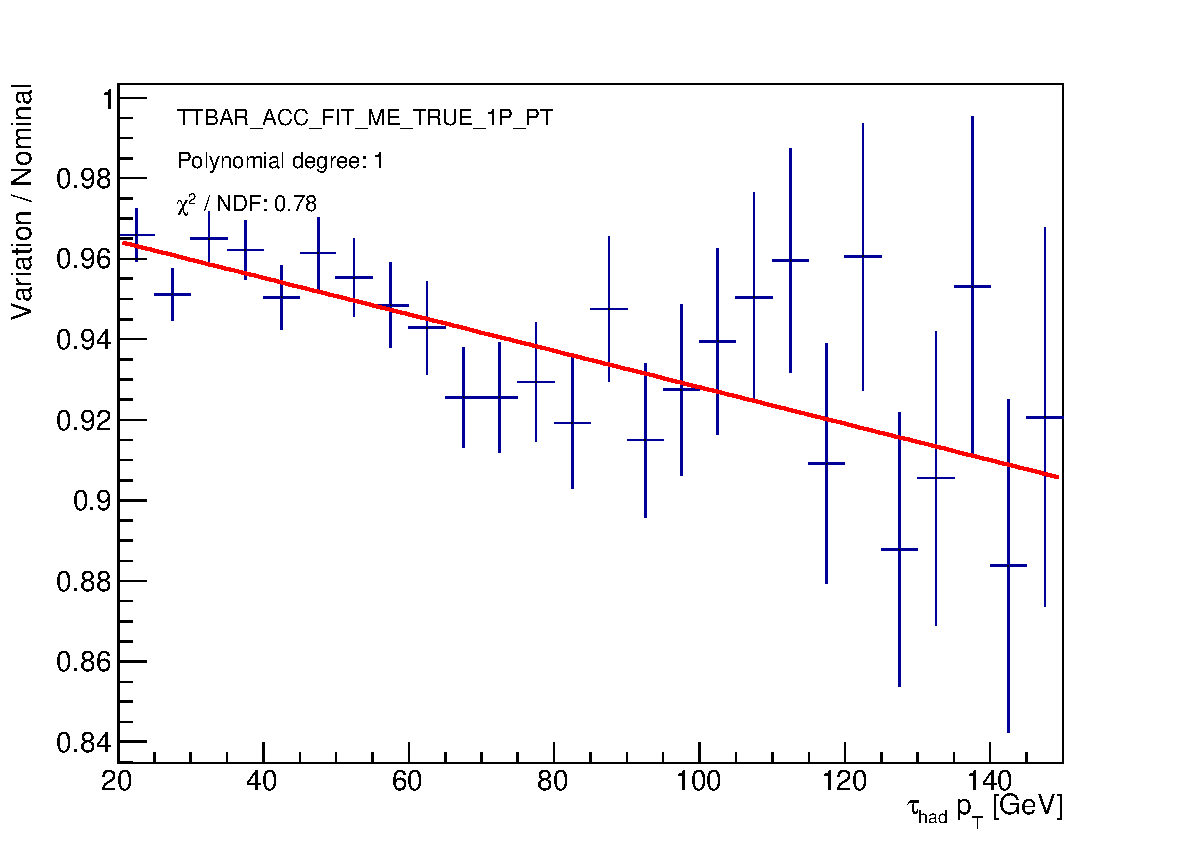
\includegraphics[width=0.49\textwidth]{figures/bkg/hadhad_ttbar_fakes/scale_factor_method/TTBAR_ACC_FIT_ME_TRUE_1P_PT}}
  \subfloat[]{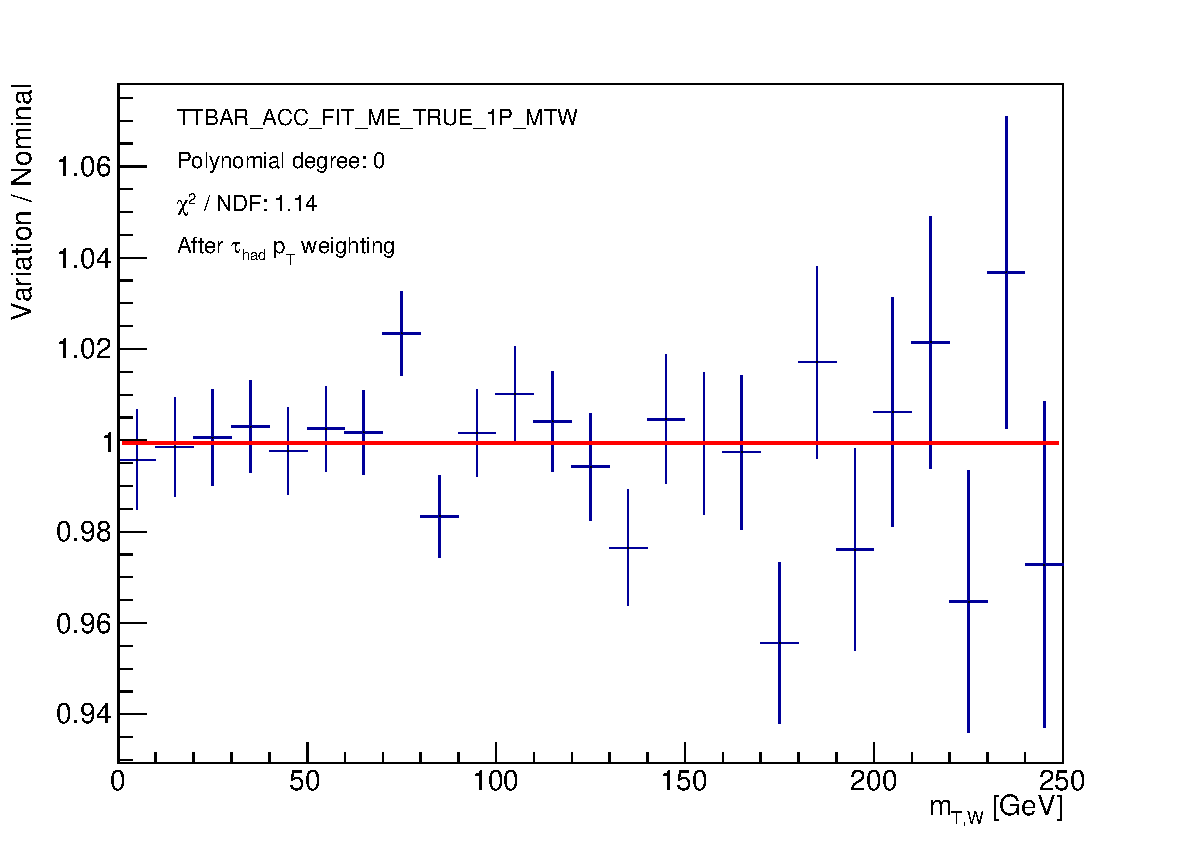
\includegraphics[width=0.49\textwidth]{figures/bkg/hadhad_ttbar_fakes/scale_factor_method/TTBAR_ACC_FIT_ME_TRUE_1P_MTW}}
  \caption{Parametrization of ME (comparing to aMCAtNLO) \ttbar
    modelling uncertainties for true 1-prong \tauhad in \tauhad \pT
    (a) and in \mtw after accounting for \tauhad \pT differences (b).}
  \label{fig:ttbarfake_hadhad_ttbar_modelling}
\end{figure}

The post-fit nuisance parameters of the SF fit for both offline loose
\tauhad identification only, and offline +
\verb|HLT_tau25_medium1_tracktwo| are shown
in~\Cref{fig:ttbarfake_hadhad_nps}. Most nuisance parameters are
compatible with their nominal value. Some pulls are observed for
\ttbar acceptance uncertainties showing consistency with the
previously observed mismodelling of \ttbar in the $b\bar{b}\tau\tau$
final state (e.g.\ in the fake rate method). Slight pulls and
constraints are observed for the \tauhad energy scale. This is
expected due to the binning of the SF measurement in \tauhad \pT and
\tauhad prong combined with the large accessible momentum range in
\ttbar as compared to the Z tag-and-probe TES measurement.

\begin{figure}[htbp]
  \centering
  \subfloat[]{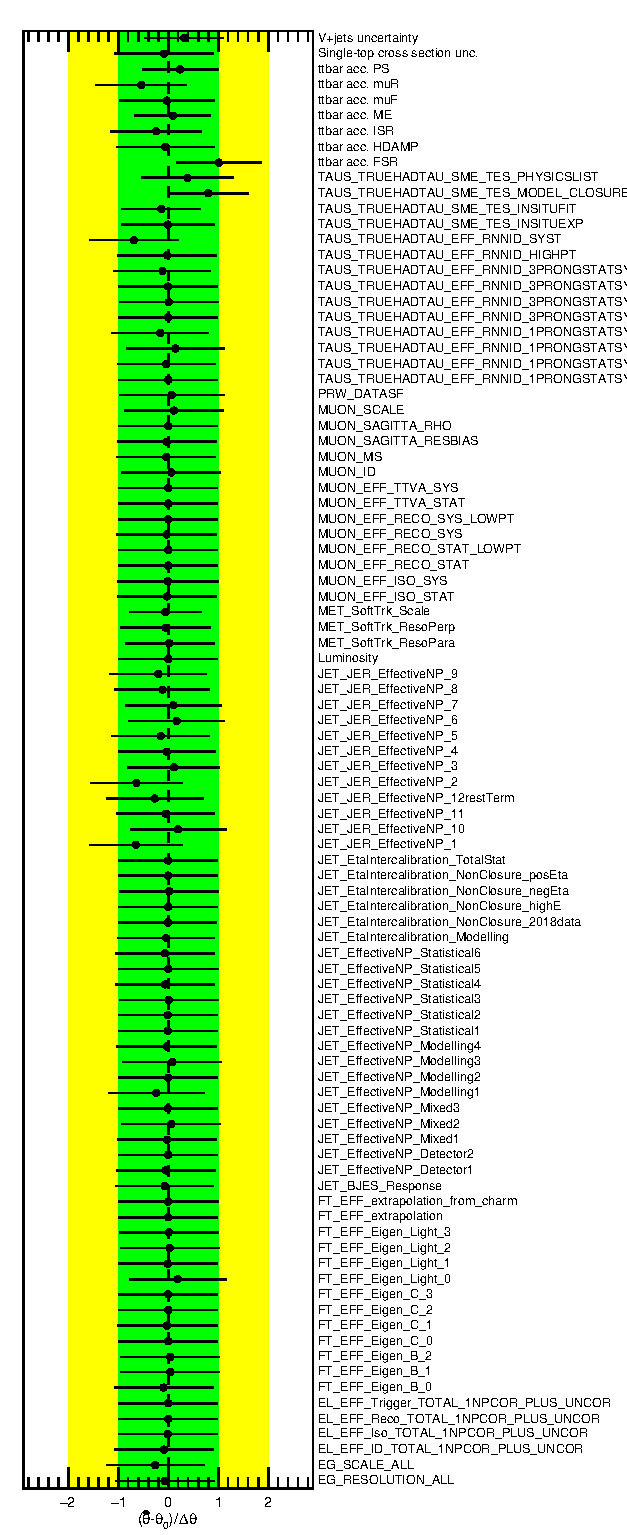
\includegraphics[width=0.42\textwidth]{figures/bkg/hadhad_ttbar_fakes/scale_factor_method/NuisPar_offl}}
  \subfloat[]{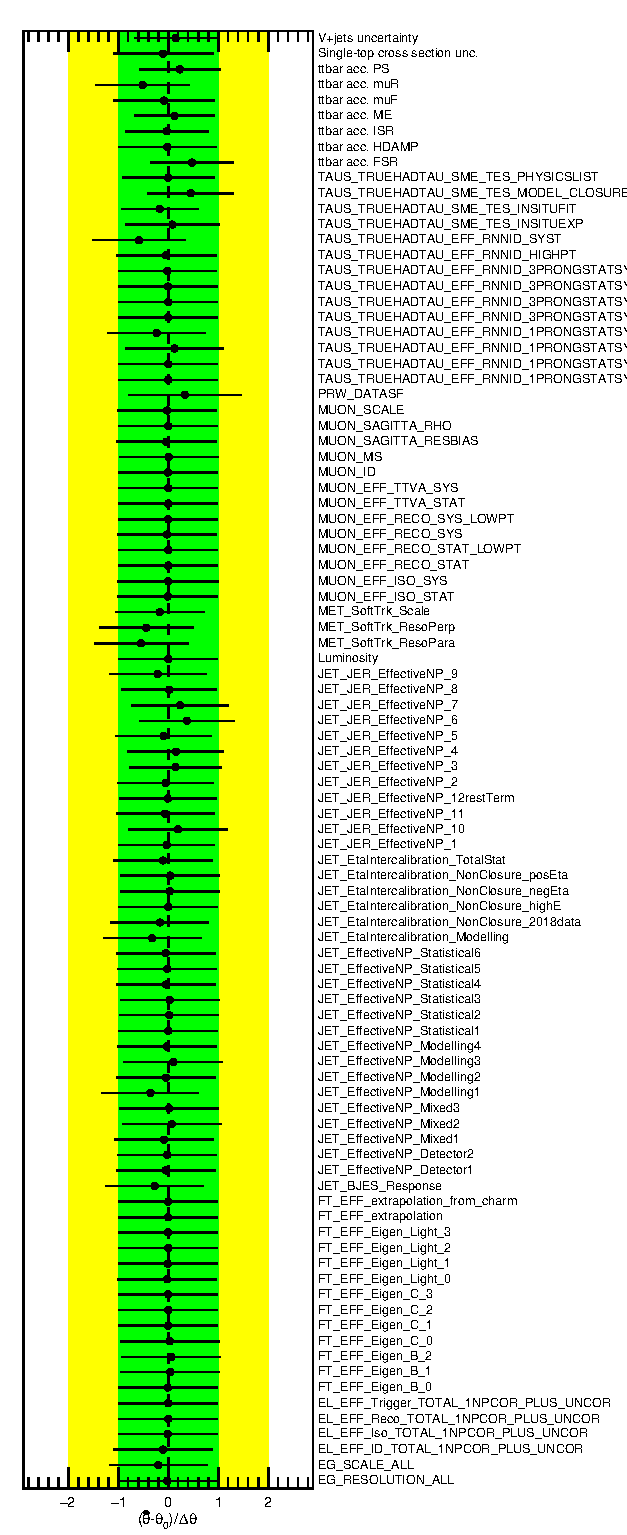
\includegraphics[width=0.42\textwidth]{figures/bkg/hadhad_ttbar_fakes/scale_factor_method/NuisPar_tau25}}
  \caption{Nuisance parameters of the offline loose (a) and loose +
    \texttt{HLT\_tau25\_medium1\_tracktwo} fake \tauhad \ttbar scale
    factor fit (b).}
  \label{fig:ttbarfake_hadhad_nps}
\end{figure}

More diagnostic plots concerning the SF measurement can be found
in~\Cref{subsec:appendix_bkg_ttbar_fake_sf}.

The measured fake \tauhad SFs are summarized
in~\Cref{fig:ttbarfake_hadhad_sf_scale_factors}. A comparison of the
scale factor approach to the fake rate approach is shown
in~\Cref{subsec:appendix_bkg_ttbar_fake_sf}
(\Cref{fig:ttbar_hadhad_sf_comparison_fr}).

\begin{figure}[htbp]
  \centering
  \subfloat[]{\includegraphics[width=0.45\textwidth]{figures/bkg/hadhad_ttbar_fakes/scale_factor_method/sf_1prong}}
  \subfloat[]{\includegraphics[width=0.45\textwidth]{figures/bkg/hadhad_ttbar_fakes/scale_factor_method/sf_3prong}}

  \subfloat[]{\includegraphics[width=0.45\textwidth]{figures/bkg/hadhad_ttbar_fakes/scale_factor_method/sf_1prong_trigger_tau25}}
  \subfloat[]{\includegraphics[width=0.45\textwidth]{figures/bkg/hadhad_ttbar_fakes/scale_factor_method/sf_3prong_trigger_tau25}}

  \caption{Comparison of fake \tauhad scale factors measured using the
    SF-method for 1-prong \tauhad (a,c) and 3-prong \tauhad (b,d) for
    all trigger setups used by the $\tauhad\tauhad$-channel.}
  \label{fig:ttbarfake_hadhad_sf_scale_factors}
\end{figure}

A summary of post-fit agreement in the regions used for the scale
factor measurement is shown
in~\Cref{fig:ttbarfake_hadhad_sf_postfit_summary}. 

\begin{figure}[htbp]
  \centering
  \subfloat[]{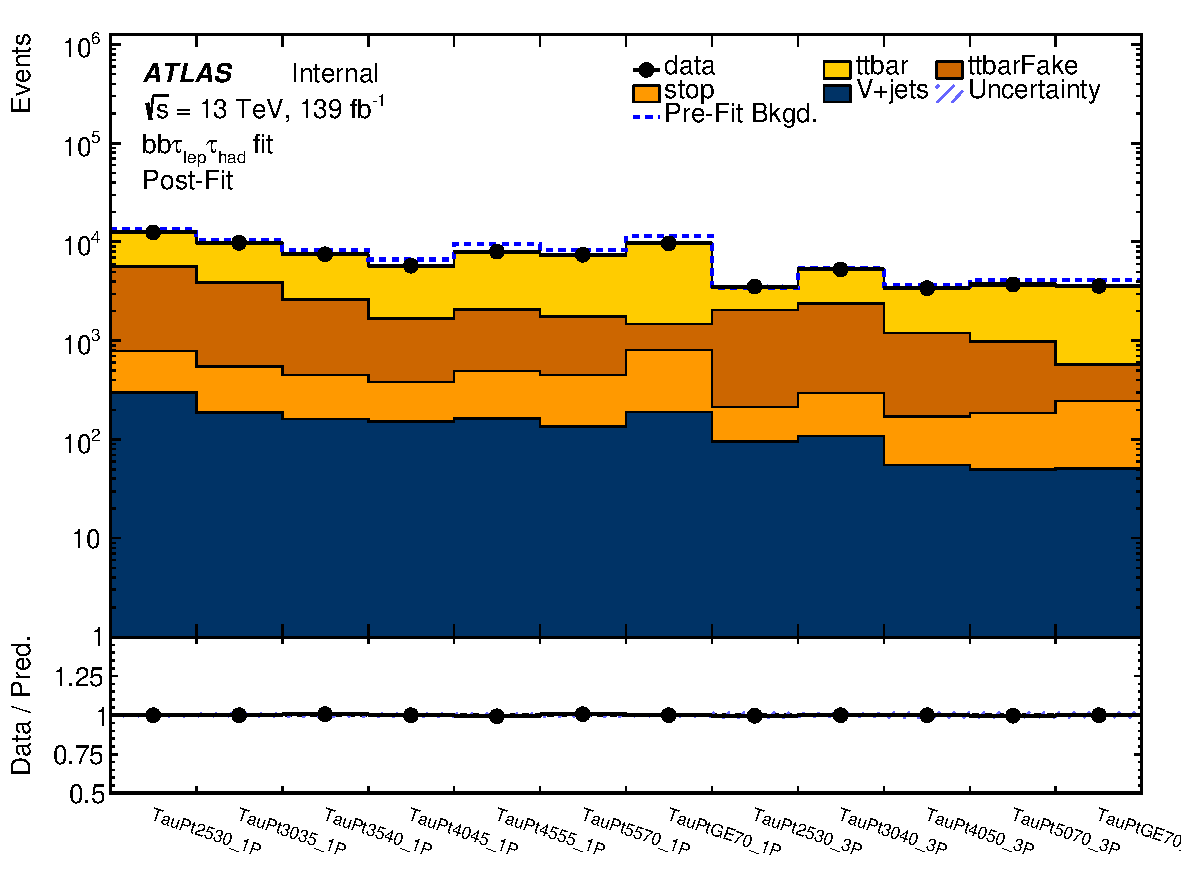
\includegraphics[width=0.45\textwidth]{figures/appendix/bkg/HadHad/ttbarSF/postfit/offl/Summary_postFit}}
  \subfloat[]{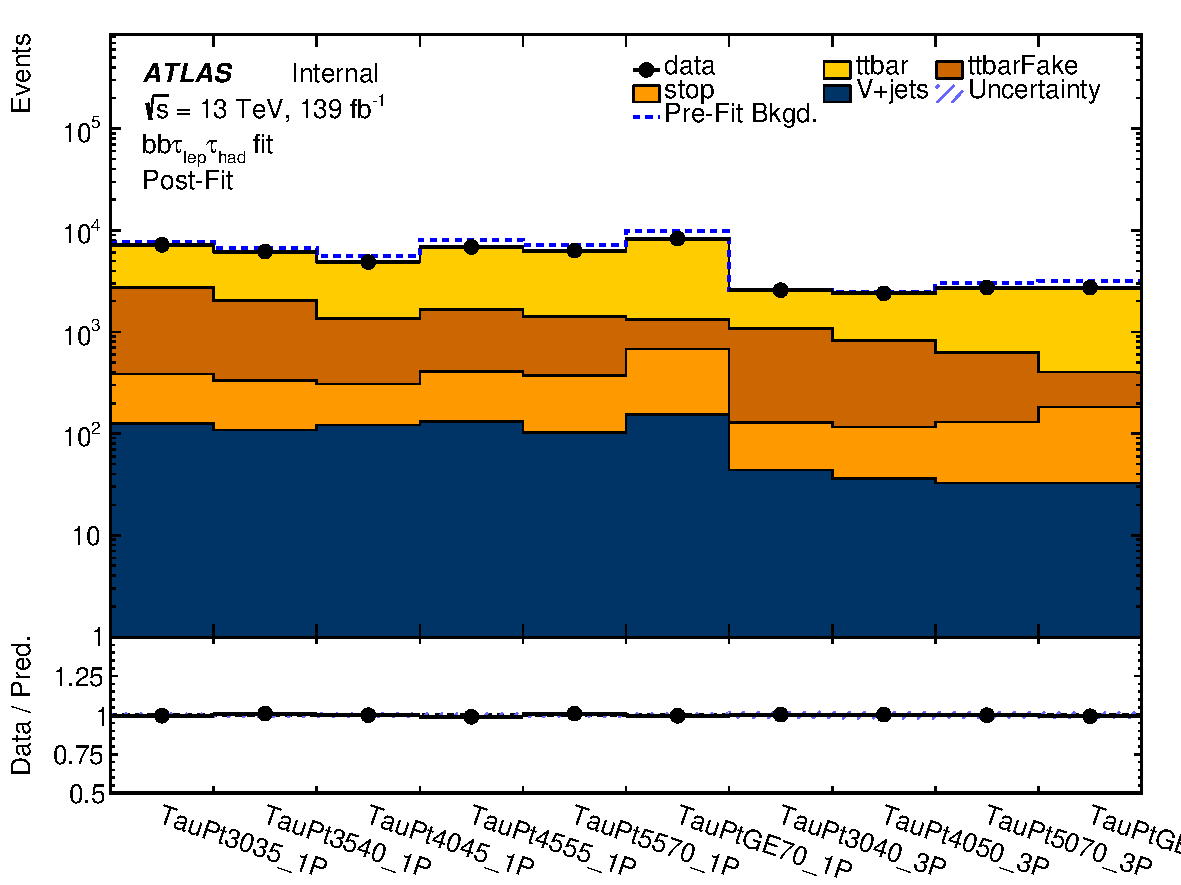
\includegraphics[width=0.45\textwidth]{figures/appendix/bkg/HadHad/ttbarSF/postfit/tau25/Summary_postFit}}

  \subfloat[]{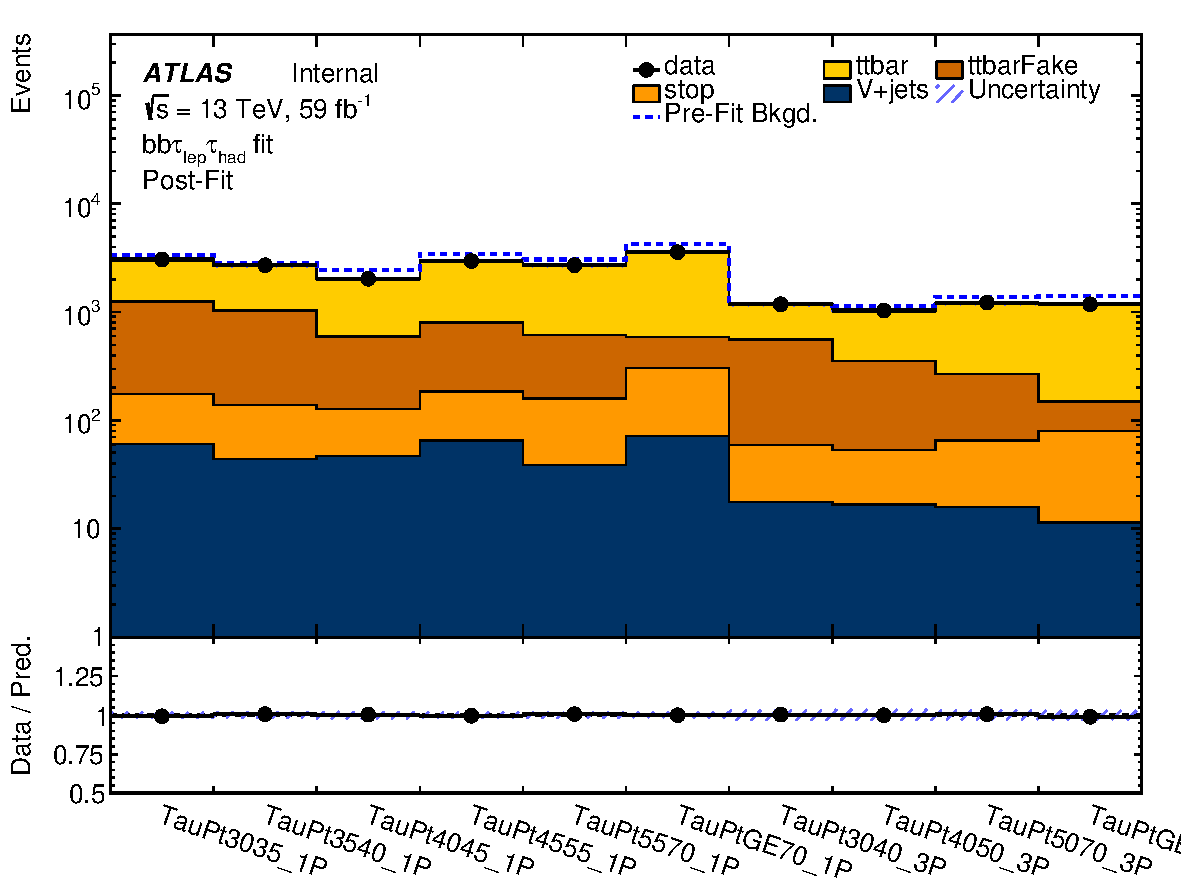
\includegraphics[width=0.45\textwidth]{figures/appendix/bkg/HadHad/ttbarSF/postfit/tau25ef/Summary_postFit}}
  \subfloat[]{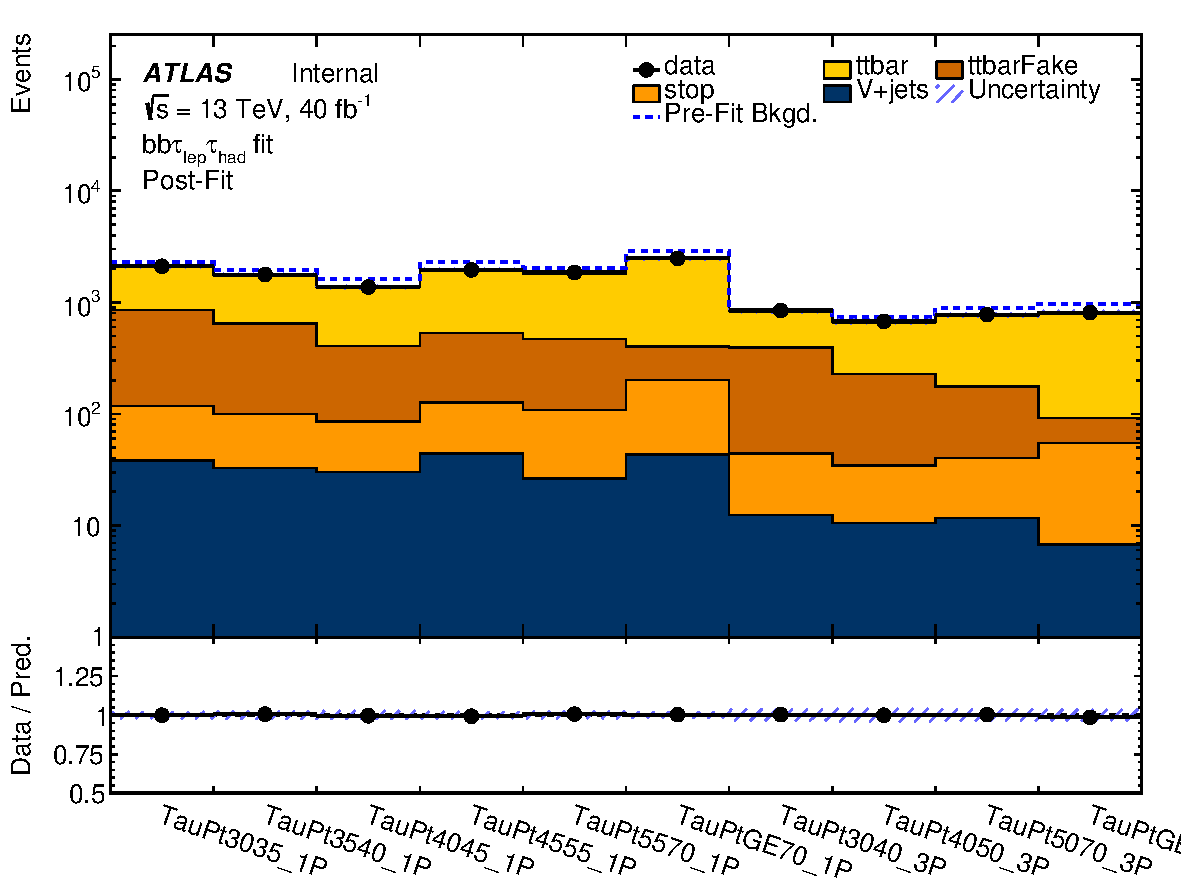
\includegraphics[width=0.45\textwidth]{figures/appendix/bkg/HadHad/ttbarSF/postfit/tau25rnn/Summary_postFit}}
  \caption{Summary of post-fit yields per region used for the fake
    \tauhad scale factor measurement. (a) Offline \tauhad
    identification only, (b) Offline + HLT\_tau25\_medium1\_tracktwo,
    (c) Offline + HLT\_tau25\_medium1\_tracktwoEF, (d) Offline +
    HLT\_tau25\_mediumRNN\_tracktwoMVA.}
  \label{fig:ttbarfake_hadhad_sf_postfit_summary}
\end{figure}

The presence of systematic uncertainties and a floating \ttbar
normalisation as well as the limited discrimination power between
\ttbar with true and fake \tauhad introduces large correlations
between the fitted scale factors
(c.f.~\Cref{fig:ttbarfake_hadhad_sf_correlation}). To not
underestimate the uncertainties, it is important that these
correlations are propagated to the final background estimate in the
$\tauhad\tauhad$-channel. This is done by performing a decomposition
of the covariance matrix returned by the fit into eigenvalues and unit
eigenvectors in SF-space. The eigenvectors describe a rotated frame in
which the scale factors\footnote{In the rotated frame the scale
  factors are represented by linear combinations of the original scale
  factors.}  have vanishing covariance with respect to any other scale
factor. The unit eigenvectors are multiplied by the standard
deviation, as given by the covariance matrix in the rotated frame, to
define (eigen-)variations of the measured scale factors that can be
treated as independent nuisance parameters in the $\tauhad\tauhad$ SR
fit. Three exemplary eigenvariations are shown
in~\Cref{fig:ttbar_hadhad_sf_eigenvariations}. The eigenvariations are
ordered in descending explained variance, i.e.\ the first variation
\texttt{EIGEN0} explains most of the variance in the SF measurement. A
total of 42 nuisance parameters\footnote{A total 12 nuisance
  parameters for the offline ID only scale factors (7 bins for 1-prong
  \tauhad and 5 bins for 3-prong \tauhad) and 10 nuisance parameters
  each for the three combinations of offline and trigger-level \tauhad
  identification (the lowest \pT bins are removed becauase they fall
  below the offline \pT-thresholds). The nuisance parameters
  (eigenvariations) are treated as independent in the final signal
  extraction fit.}  are provided for the final fit most of which have
negligible impact and will be pruned during the statistical
analysis. An example of the decomposition is shown
in~\Cref{fig:ttbar_hadhad_sf_eigenvariations}.

\begin{figure}[htbp]
  \centering
  \includegraphics[width=0.5\textwidth]{figures/bkg/hadhad_ttbar_fakes/scale_factor_method/CorrMatrixSlice}
  \caption{Correlation between measured scale factors and the \ttbar
    normalisation for the offline \tauhad-ID only fit.}
  \label{fig:ttbarfake_hadhad_sf_correlation}
\end{figure}

\begin{figure}[htbp]
  \centering
  \subfloat[]{\includegraphics[width=0.49\textwidth]{figures/bkg/hadhad_ttbar_fakes/scale_factor_method/sf_variations_1p}}
  \subfloat[]{\includegraphics[width=0.49\textwidth]{figures/bkg/hadhad_ttbar_fakes/scale_factor_method/sf_variations_3p}}
  \caption{Eigenvariations of the measurement of fake \tauhad scale
    factors for loose offline \tauhad-ID and
    HLT\_tau25\_medium1\_tracktwo for 1-prong (a) and 3-prong
    (b). Three varations are shown: \texttt{EIGEN0} \& \texttt{EIGEN1}
    explaining the majority and \texttt{EIGEN9} explaining the least
    amount of variance.}
  \label{fig:ttbar_hadhad_sf_eigenvariations}
\end{figure}

To estimate the \ttbar background with fake \tauhad in the
$\tauhad\tauhad$-channel, scale factors are applied to fake \tauhad
(i.e.\ \tauhad not truth-matched to leptons) from \ttbar MC passing
loose identification and, if applicable, trigger-matching. The set of
scale factors is picked according to the trigger-channel and random
run number of the event mirroring the trigger selection described
in~\Cref{sec:hadhad_trigger_selection}. For single \tauhad trigger
events, the scale factors corresponding to HLT\_tau25 are applied to a
leading fake \tauhad and the offline ID only scale factors to
subleading fake \tauhad. For di-\tauhad trigger events, the HLT\_tau25
scale factors to leading and subleading fake \tauhad. A comparison of
uncorrected fakes and scale factor corrected fakes from \ttbar MC can
be found in~\Cref{fig:ttbar_hadhad_sf_background_estimate}
in~\Cref{subsec:appendix_bkg_ttbar_fake_sf}. Considering statistical
and systematic uncertainties, no large differences are observed
between the scale factor corrected and uncorrect \tauhad fakes from
simulation. However, the scale factor estimate will still be used as
it provides a measurement-driven estimate of uncertainties on the fake
\tauhad modelling in \ttbar.

When applying the scale factors to events in the
$\tauhad\tauhad$-channel, an approach similar to the application of
true \tauhad calibrations (e.g.\ trigger and offline \tauhad), where
it is assumed that the calibrations factorize in a multi-\tauhad final
state, is taken. In this analysis this assumption only affects the
\ttbar final state with two fake \tauhad (FF events). This
contribution is a subleading source of fake \tauhad making up only
15\,\% of the total \ttbar+fake \tauhad contribution (the dominant
contributions are events where only one \tauhad is fake -- i.e.\ TF
and FT events). The uncertainties related to the fake scale factor
measurement are assumed to be fully correlated between both \tauhad in
DTT FF events\footnote{For the negligible contribution of FF STT
  events the scale factors for the leading and the subleading \tauhad
  are assumed to be uncorrelated.} and are propagated as such to the
final background estimate in the \hadhad-channel. Compared to the size
of the uncertainties affecting FF events (e.g.\ 40 \% for the
$\lephad \ra \hadhad$ extrapolation uncertainties, c.f.\
\Cref{tab:ttbar_fake_sf_extrapol_ff}), deviations from this assumption
are thought to be negligible.

Additional plots relating to the scale factor measurement and
application can be found in~\Cref{subsec:appendix_bkg_ttbar_fake_sf}.

To account for the differences between the SF measurement region and
the application region, extrapolation uncertainties are derived
accounting for the differences in acceptance between these regions.
The approach closely follows the extrapolation uncertainies derived
for the \ttbar with true \tauhad described
in~\Cref{sec:systematics_backgroundmodelling}.  Since the scale
factors are measured in bins of \tauhad \pT and prong, the acceptance
differences are checked dependent on these quantities.

The fake \tauhad \pT and prong dependency is checked for events
containing exactly one \tauhad being faked by a jet. Except for the
variation of the parton shower, no significant \pT dependency was
found. Uncertainties only affecting the normalization are summarized
in~\Cref{tab:ttbar_fake_sf_extrapol_uncertainties}. The impact of the
parton shower variations, shown
in~\Cref{fig:ttbar_fake_sf_extrapol_psshape}, is parametrized using
polynomial interpolation in \tauhad \pT separately for 1- and 3-prong
\tauhad.

\begin{table}[htb]
  \centering

  \begin{tabular}{lrr}
    \toprule
    Source & Uncertainty (1-prong) & Uncertainty (3-prong)\\
    \midrule
    ME & $\pm 1.7 \%$ & $\pm 6.0 \%$ \\
    PS & -- & -- \\
    $h_\text{damp}$ & $\pm 1.6 \%$ & $\pm 8.2 \%$ \\
    $\mu_\text{F}$ & $\pm  0.2 \%$ & $\pm 0.3 \%$ \\
    $\mu_\text{R}$ & $\pm 0.04 \%$ &  $\pm 0.5 \%$ \\
    ISR & $\pm 0.3 \%$ & $\pm 0.8 \%$ \\
    FSR & $\pm 4.0 \%$ & $\pm 8.5 \%$ \\
    \midrule
    Total & $\pm 4.7 \%$ & $\pm 13.3 \%$\\
    \bottomrule
  \end{tabular}
  \caption{Extrapolation uncertainties derived by comparing the impact
    of variations in \ttbar modelling on the acceptance times
    efficiency ($\mathcal{A} \times \varepsilon$) ratio between the
    \hadhad SR and the \lephad Top/SF-CR. The parton shower variation
    has non-negligible effect on the \tauhad \pT shape and is
    therefore treated separately.}
  \label{tab:ttbar_fake_sf_extrapol_uncertainties}
\end{table}

\begin{figure}[htbp]
  \centering

  \subfloat[]{\includegraphics[width=0.33\textwidth]{figures/bkg/hadhad_ttbar_fakes/scale_factor_method/extrapolation_tf_ft/fit_me_1p}}
  \subfloat[]{\includegraphics[width=0.33\textwidth]{figures/bkg/hadhad_ttbar_fakes/scale_factor_method/extrapolation_tf_ft/fit_ps_1p}}
  \subfloat[]{\includegraphics[width=0.33\textwidth]{figures/bkg/hadhad_ttbar_fakes/scale_factor_method/extrapolation_tf_ft/fit_hdamp_1p}}

  \subfloat[]{\includegraphics[width=0.33\textwidth]{figures/bkg/hadhad_ttbar_fakes/scale_factor_method/extrapolation_tf_ft/fit_me_3p}}
  \subfloat[]{\includegraphics[width=0.33\textwidth]{figures/bkg/hadhad_ttbar_fakes/scale_factor_method/extrapolation_tf_ft/fit_ps_3p}}
  \subfloat[]{\includegraphics[width=0.33\textwidth]{figures/bkg/hadhad_ttbar_fakes/scale_factor_method/extrapolation_tf_ft/fit_hdamp_3p}}
  \caption{Dependence of fake \tauhad extrapolation uncertainties on
    \tauhad \pT and prong for the variation of the matrix element (a,
    d), the parton shower (b, e) and the damping parameter
    $h_\text{damp}$ (c,f) for 1-prong \tauhad (top row) and 3-prong
    \tauhad (bottom row). The variation of the matrix element and
    damping parameter is consistent with a normalization
    difference. The variation of the parton shower leads to shape
    effects in \tauhad \pT which are parametrized using polynomial
    interpolation.}
  \label{fig:ttbar_fake_sf_extrapol_psshape}
\end{figure}

The extrapolation uncertainty for \ttbar with two fake \tauhad, making
up less than 14 \% of the total \ttbar background with at least one
fake \tauhad and less than 4 \% of the total background, cannot be
related between the measurement and signal region based on fake
\tauhad properties without introducing ambiguities due to the
different final states (i.e.\ comparison of a single fake \tauhad
final state to a two fake \tauhad final state). Given the small
contribution of this background to the total fake \tauhad from \ttbar
background, any shape effects will be heavily dilluted. Therefore, the
extrapolation uncertainties for this minor contribution is treated
inclusively in the properties of the fake \tauhad. The uncertainty is
summarized in~\Cref{tab:ttbar_fake_sf_extrapol_ff}. Additionally, the
impact of the \ttbar modelling uncertainties on the MVA input
variables are checked. Shape differences in these variables are only
observed for the variation of the parton shower but they remain
negligible when considering the small contribution of the two fake
\tauhad background and the large extrapolation uncertainty of
\SI{35}{\percent} already being assigned due to the parton shower
(c.f.~\Cref{tab:ttbar_fake_sf_extrapol_ff}). Additional information
can be found in~\Cref{fig:ttbar_fake_sf_ff_ps_shapes}.

\begin{table}[htbp]
  \centering
  \begin{tabular}{lr}
    \toprule
    Source & Uncertainty \\
    \midrule
    ME & $\pm 9.2 \%$ \\[0.2em]
    PS & $\pm 35 \%$ \\[0.2em]
    $h_\text{damp}$ & $\pm 4.6 \%$ \\[0.2em]
    $\mu_\text{R}$ & $\substack{+0.43 \% \\ -0.34 \%}$ \\[0.2em]
    $\mu_\text{F}$ & $\substack{+0.06 \% \\ -0.09 \%}$ \\[0.2em]
    ISR & $\substack{+0.05 \% \\ -0.45 \%}$ \\[0.2em]
    FSR & $\substack{+18 \% \\ -6.8 \%}$ \\[0.2em]
    \midrule
    Total & $\substack{+41 \% \\ -38 \%}$ \\[0.2em]
    \bottomrule
  \end{tabular}
  \caption{Extrapolation uncertainties, inclusive in fake \tauhad \pT
    and prong, for \ttbar where both \tauhad are faked by jets. The
    uncertainty is derived by comparing the acceptance times
    efficiency ratio between the \hadhad application region and the
    \lephad SF measurement region for different variations in \ttbar
    modelling.}
  \label{tab:ttbar_fake_sf_extrapol_ff}
\end{table}


\FloatBarrier
\subsubsection{Anti-ID Region Scale Factors}
\label{sssec:ttbar_fake_sf_antiid}

When estimating the multi-jet fakes using the fake factor method
(cf.~\Cref{subsec:HadHadmultijet}), a large fraction of \ttbar
containing at least one fake \tauhad needs to be subtracted in the
2-tag OS Anti-ID region when estimating the multi-jet contribution in
the $\tauhad\tauhad$ SR. To estimate an uncertainty on this
subtraction, which makes up the majority of the non-multi-jet
background subtraction, an additional set of fake \tauhad SFs is
measured for the Anti-ID region.

The Anti-ID SF measurement uses the same CR definition except for
inverting the offline \tauhad identification requirement by requiring
the \tauhad to fail the loose \tauhad identification working point but
fulfilling the $\text{RNN} > 0.01$ requirement of the Anti-ID region.
The requirements on trigger-matching for the SF measurement remain
unchanged. The scale factor measurement for the Anti-ID region closely
follows the approach taken for the ID-region measurement. The
differences from the ID-region fit are outlined in the following.

The inversion of the \tauhad identification requirement rejects most
\ttbar with a true \tauhad while being efficient at selecting \ttbar
with a \tauhad originating from jets. A summary of the yields per
region is shown in~\Cref{fig:ttbar_hadhad_sf_antitau_region_summary}
with offline identification requirements only as well as offline + HLT
identification requirements. Due to the small fraction of \ttbar with
true \tauhad, no strong constraint on the \ttbar normalization can be
extracted in the fit. This further increases the correlations between
the measured scale factors as compared to the ID-region SF
measurement.

\begin{figure}[htbp]
  \centering

  \subfloat[]{\includegraphics[width=0.45\textwidth]{figures/bkg/hadhad_ttbar_fakes/scale_factor_method/anti_tau/offl/Summary}}
  \subfloat[]{\includegraphics[width=0.45\textwidth]{figures/bkg/hadhad_ttbar_fakes/scale_factor_method/anti_tau/tau25/Summary}}

  \caption{Pre-fit summary of regions entering the \ttbar fake scale
    factor measurement for Anti-ID (a) and Anti-ID +
    HLT\_tau25\_medium1\_tracktwo (b).}
  \label{fig:ttbar_hadhad_sf_antitau_region_summary}
\end{figure}

A reduced set of experimental systematics is used for the measurement
due to size limitations of the CxAODs with the Anti-ID selection. As a
result, only weight systematics and variations of the tau energy scale
are considered in this measurement. Variations affecting the
4-momentum of other reconstructed objects are neglected. The
difference of the measured SFs to 1 is introduced as an additional
uncertainty to account for the lack of 4-momentum uncertainties when
applying the Anti-ID SFs for the subtraction in the fake factor
estimation of the multi-jet background. The theoretical and two-point
modelling uncertainties from the ID region are also used for the
Anti-ID region fits\footnote{The two-point modelling uncertainties are
  not expected to depend on the identification level of the \tauhad
  aside from a shaping of the \tauhad \pT distribution with different
  identification requirements. The parametrizations of two-point
  systematics are provided differentially in \tauhad \pT and can
  therefore be also used in the Anti-ID region.}. The post-fit
nuisance parameters for all four fits are depicted
in~\Cref{fig:ttbarfake_hadhad_nps_antitau}.

\begin{figure}[htbp]
  \centering
  \subfloat[]{\includegraphics[width=0.4\textwidth]{figures/bkg/hadhad_ttbar_fakes/scale_factor_method/anti_tau/offl/NuisPar}}
  \subfloat[]{\includegraphics[width=0.4\textwidth]{figures/bkg/hadhad_ttbar_fakes/scale_factor_method/anti_tau/tau25/NuisPar}}

  \subfloat[]{\includegraphics[width=0.4\textwidth]{figures/bkg/hadhad_ttbar_fakes/scale_factor_method/anti_tau/tau25ef/NuisPar}}
  \subfloat[]{\includegraphics[width=0.4\textwidth]{figures/bkg/hadhad_ttbar_fakes/scale_factor_method/anti_tau/tau25rnn/NuisPar}}

  \caption{Nuisance parameters of the Anti-ID (a), Anti-ID +
    \texttt{HLT\_tau25\_medium1\_tracktwo} (b), Anti-ID +
    \texttt{HLT\_tau25\_medium1\_tracktwoEF} (c), and Anti-ID +
    \texttt{HLT\_tau25\_medium1\_tracktwoEF} \textbf{or}
    \texttt{HLT\_tau25\_mediumRNN\_tracktwoMVA} fake \tauhad \ttbar
    scale factor fit (d).}
  \label{fig:ttbarfake_hadhad_nps_antitau}
\end{figure}

The measured Anti-ID scale factors are shown
in~\Cref{fig:ttbar_hadhad_sf_antitau}. With the looser \tauhad
identification requirement, the measured fake \ttbar scale factors are
close to unity with the same trend of a decreasing SF with increasing
\tauhad \pT that is also observed in the ID-region.

\begin{figure}[htbp]
  \centering

  \subfloat[]{\includegraphics[width=0.45\textwidth]{figures/bkg/hadhad_ttbar_fakes/scale_factor_method/anti_tau/sf_1prong}}
  \subfloat[]{\includegraphics[width=0.45\textwidth]{figures/bkg/hadhad_ttbar_fakes/scale_factor_method/anti_tau/sf_3prong}}

  \subfloat[]{\includegraphics[width=0.45\textwidth]{figures/bkg/hadhad_ttbar_fakes/scale_factor_method/anti_tau/sf_1prong_trigger_tau25}}
  \subfloat[]{\includegraphics[width=0.45\textwidth]{figures/bkg/hadhad_ttbar_fakes/scale_factor_method/anti_tau/sf_3prong_trigger_tau25}}

  \caption{Comparison of fake \tauhad scale factors measured using the
    SF-method for 1-prong \tauhad (a,c) and 3-prong \tauhad (b,d) for
    all trigger setups used by the $\tauhad\tauhad$-channel in the
    Anti-ID region.}
  \label{fig:ttbar_hadhad_sf_antitau}
\end{figure}

Additional plots can be found
in~\Cref{app:sssec:antiid_ttbar_fake_scale_factors}.

The scale factors are applied when subtracting \ttbar with fake
\tauhad in the 2-tag OS Anti-ID region to estimate the multi-jet
contribution in the $\tauhad\tauhad$ SR. Correlations between scale
factors are propagated using the eigendecomposition approach. The
variance of the scale factor measurement is dominated by the leading
eigenvariation due to the very large correlations (85 to 95 \%)
between scale factor bins. Therefore, only the leading variations are
kept to define the uncertainty on the fake \tauhad \ttbar subtraction
for the multi-jet estimate in the $\tauhad\tauhad$ SR. Additionally,
the full difference of the scale factors to one is assigned. The
impact on the fake estimate in the $\tauhad\tauhad$ SR is explained in
more detail in~\Cref{subsec:uncertainties_hadhamultijetfakes}.

\FloatBarrier
